\documentclass[10pt,a4paper]{article}
\usepackage[utf8]{inputenc}
\usepackage[italian]{babel}
\usepackage{amsmath}
\usepackage{amsfonts}
\usepackage{amssymb}
\usepackage{graphicx}
\usepackage[left=2cm,right=2cm,top=2cm,bottom=2cm]{geometry}
\newcommand{\rem}[1]{[\emph{#1}]}

\author{Gruppo AC \\ Federico Belliardo, Giulia Franchi, Francesco Mazzoncini}
\title{Esercitazione N.4: Amplificatore a transistor}
\begin{document}

\maketitle

\section{Scopo dell'esperienza}
L'esercitazione ha come scopo quello di realizzare un circuito amplificatore, utilizzando un transistor \textit{npn} 2N1711.

\section{Montaggio del circuito e verifica del punto di lavoro}

\begin{figure}[!htb]
  \centering
  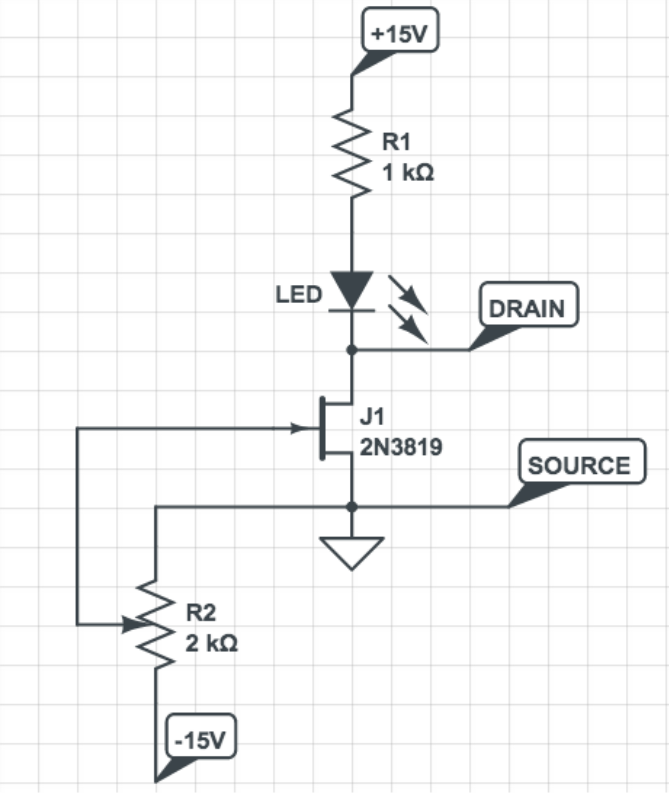
\includegraphics[scale=0.3]{circuito1.png}
\caption{Schema amplificatore a transitor.}
\label{circuito}
\end{figure}

Abbiamo montato il circuito in figura \ref{circuito} come richiesto, con: $R_1= 179\pm1  k\Omega$, $R_2= 18.0\pm0.1  k\Omega$, $R_C= 9.95\pm 0.09  k\Omega$, $R_E= 0.987\pm 0.008 \, k\Omega$, $C_{IN}= 230\pm10  nF$, $C_{OUT}= 99\pm4  nF$ e $C_E= 100\pm20  \mu F$. Tutti i componenti sono stati misurati con multimetro digitale, tranne il condensatore elettrolitico di cui abbiamo assunto il valore nominale.\\
Supponiamo che il transistor lavori in zona attiva, $V_{BE} = 0.6 \pm 0.1 \, V$. Abbiamo inoltre definito $V_{PART}=V_{CC}\frac{R_2}{R_1+R_2}$, per determinarla abbiamo prima misurato la tensione in ingresso $V_{CC}= 20.2\pm0.1 V$, così la tensione ai capi del partitore risulta $V_{PART}=1.85 \pm 0.01\,V$.


\subsection{Misura del punto di lavoro}
Per la determinazione del punto di lavoro del circuito si è misurato $V_{CE}= 7.50\pm0.04 \, V$ e la caduta di potenziale ai capi della resistenza $R_C$, $V_{R_C}= 11.62\pm0.05  V$, in modo da poter determinare $I_C=\frac{V_{RC}}{I_C} = 1.17\pm0.01\,mA$.
Confrontando questi valori misurati con i valori teorici, $I_C=\frac{V_{PART}-V_{BE}}{R_E}= 1.12\pm0.01\,mA$ e $V_{CE}=V_{CC}-(R_C+R_E)I_C= 7.4\pm0.1\,V$, si vede che si ha compatibilità entro l'errore.\\
La retta di lavoro attesa è  $V_{CC}=V_{CE}+I_C(R_C+R_E)$.


\subsection{Misura delle tensioni ai terminali del transistor}
Abbiamo misurato le tensioni $V_B= 1.77\pm0.01\,V$, $V_E= 1.17\pm0.01\,V$, $V_{BE}= 0.605\pm0.004\,V$ e $V_C= 8.47\pm0.04\,V$. Sono compatibili con quanto abbiamo calcolato teoricamente?! $V_B= V_{PART}=1.85 \pm 0.01\,V$, $V_E=I_C^Q R_E = 1.2 \pm 0.1 \,V$, $V_C=V_{CC}-I_C^Q R_C = 8 \pm 1 \, V$.


\subsection{Valutazione della corrente di base}
Ci aspetteremmo una corrente di base $I_B=\frac{I_C}{h_{FE}} = 6.9 \pm 0.4) \, \mu A$, dato che si suppone il transistor lavori in zona attiva. Misuriamo le cadute di potenziale ai capi delle resistenze $R_1$ e $R_2$, $V_{R1}= \pm V$ e $V_{R2}= \pm V$, da cui abbiamo ricavato $I_{R1} = 98.3\pm0.8 \, \mu A$ e $I_{R2} = 103.0\pm0.8 \, \mu A$, dalle quali infine abbiamo ricavato $I_B=I_{R1}-I_{R2}= 5\pm1 \,\mu A$. Il partitore è ragionevolmente \emph{stiff}.

\section{Risposta a segnali sinusoidali di frequenza fissa}
In questa parte dell'esperienza si è utilizzato un segnale ad una frequenza fissa pari a $f= 5.00\pm0.05 \, kHz$.

\subsection{Misura del guadagno in tensione}
Abbiamo preso diverse misure di $V_{OUT}$ (è dello sfasamento di tempo rispetto all'ingresso) in funzione di $V_{IN}$ al variare di quest'ultimo, prestando attenzione ai fenomeni di clipping. Nella tabella \ref{ampiezza} seguenze riportiamo le nostre misure, aggiungendo anche il calcolo del guadagno in tensione, $A_V=\frac{V_{OUT}}{V_{IN}}$ e dello sfasamento angolare rispetto a $\pi \,rad$.\\
L'oscilloscopio è stato utilizzato in modalità AC.\\
Tutti i dati mostrati nelle tabelle e nei grafici (in tutta la relazione) riportano sia l'errore sistematico che che quello statistico sommati in quadratura, in tutti i fit e le propagazioni sono stati considerati gli errori statistici.

\begin{table}[!hbt]
\centering
\begin{tabular}{|c|c|c|c|c|c|c|c|}
\hline 
$V_{IN}$ [V] & $\sigma V_{IN}$ [V] & $V_{OUT}$ [V]& $\sigma V_{OUT}$ [V] & $\phi - \pi$ [rad] & $\sigma \phi$ [rad] & $A_V$ & $\sigma A_V$ \\ 
\hline
0.206 & 0.006 & 2.00 & 0.06 & 0.06 & 0.07 & 9.7 & 0.1\\
0.294 & 0.009 & 2.86 & 0.09 & 0.06 & 0.07 & 9.73 & 0.08\\
0.42 & 0.01 & 2.00 & 0.06 & 0.09 & 0.07 & 4.76 & 0.05\\
0.51 & 0.02 & 5.0 & 0.2 & 0.06 & 0.07 & 9.84 & 0.05\\
0.62 & 0.02 & 6.0 & 0.2 & 0.03 & 0.07 & 9.61 & 0.04\\
0.71 & 0.02 & 6.9 & 0.2 & 0.06 & 0.07 & 9.66 & 0.04\\
0.80 & 0.02 & 7.7 & 0.2 & 0.06 & 0.07 & 9.60 & 0.05\\
0.90 & 0.03 & 8.7 & 0.3 & 0.09 & 0.07 & 9.73 & 0.06\\
1.03 & 0.03 & 9.9 & 0.3 & 0.06 & 0.07 & 9.63 & 0.05\\
1.12 & 0.03 & 10.6 & 0.3 & 0.03 & 0.07 & 9.46 & 0.05\\
1.21 & 0.04 & 11.5 & 0.3 & 0.09 & 0.07 & 9.50 & 0.05\\
1.30 & 0.04 & 12.6 & 0.4 & 0.06 & 0.07 & 9.69 & 0.04\\
\hline
\end{tabular}
\caption{Misure di tensione, guadagno e fase.} \label{ampiezza}
\end{table}
Si può vedere come il segnale in uscita sia sfasato di $\pi \, rad$ come atteso dai calcoli teorici. Tutte le misure dello sfasamento sono compatibili con zero entro l'errore sperimentale. Tuttavia si può osservare una fase sistematicamente maggiore di $\pi \, rad$ probabilmente a causa dell'impedenza dei condensatori in ingresso e uscita. Il valore medio dell'attenuzione (con errore propagato in maniera statistica sulla media di tutte le misure) è: $A = (-9.24 \pm 0.02)$.

La tensione misurata a cui inizia il \emph{clipping} inferiore è circa $V_{inf} = 1.4 \,V$, mentre il clipping superiore inizia circa a $V_{sup} = 2.2 \, V$. Per referenza si gurdi l'immagine \ref{clipping}.\\
Questo è dovuto al fatto che il punto di quiescenza scelto è più vicino alla zona di saturazione che alla zona di interdizione. Il clipping inferiore corrisponde alla zona di saturazione, perchè significa che $V_{IN}$ ha il valore massimo e quindi la corrente di base è tale da mandare il transistor in saturazione.\\
Quando si ha clipping superiore la $V_{IN}$ è al minimo valore dunque non ho polarizzazione della base e sono in interdizione.
Entrambi gli effetti accennati sono effetti non lineari del transistor, cioè deviazioni dal comportamento ideale in cui vengono mandati segnale armonici in segnali armonici.\\

\begin{figure}[!htb]
  \centering
  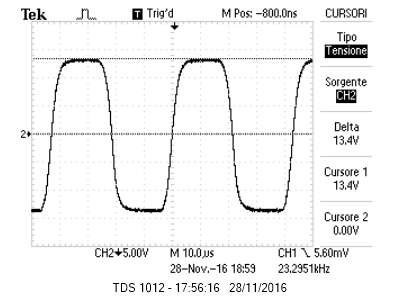
\includegraphics[scale=1.0]{clipping.png}
\caption{Schema amplificatore a transitor.}
\label{clipping}
\end{figure}

\subsection{Impedenza di ingresso del circuito}
Come impedenza in ingresso del circuito ci aspettiamo $R_{IN}=R_1//R_2//(h_{ie}+h_{fe}R_E) = 15.3\pm0.1$.
Abbiamo misurato la tensione in uscita del circuito in Fig \ref{circuito}: $V_{OUT,1} = (6.44\pm0.02) \, V$, e successivamente abbiamo inserito una resistenza, $R_S= (18.1\pm0.1) \, k\Omega$, fra il generatore e $C_{IN}$, misurando poi $V_{OUT,2}= (2.94 \pm 0.02) \, V$. Il valore di $V_{IN} = (668 \pm 2) \, mV$, che rimane costante durate le due misure. Utilizzando la formula $\frac{R_S}{R_{IN}}=\frac{V_{OUT,1}}{V_{OUT,2}}-1$ ci è stato possibile ricavare il valore dell'impedenza in ingresso, $R_{IN}= 15.2\pm0.2\, k\Omega$. 
Per il calolo della resistenza di ingresso teorica la resistenza dinamica della giunzione è stata stimata dalla misure prese assumendo il coefficiente $h_{fe} = 170\pm10$ determinato nella scorsa esperienza. Si ottiene un accordo ottimo della misura e della stima teorica

\subsection{Impedenza di uscita del circuito}
Come impedenza di uscita del circuito ci aspettiamo $R_{OUT}= R_C = 9.95\pm0.09\, k\Omega$. Come in precedenza abbiamo effettuato due misure di tensione: la prima con il circuito di partenza, $V_{OUT,1}= (6.40\pm0.02) \, V$, la seconda è stata presa misurata dopo aver inserito tra l'uscita e la massa una resistenza di carico $R_L = (10.05 \pm 0.08) \, k\Omega$, $V_{OUT,2}= (3.62\pm0.02)\,V$. La tensione in ingresso è: $V_{IN} = 664 \pm 2 \,$. Grazie alla formula $\frac{R_{OUT}}{R_{L}}=\frac{V_{OUT,1}}{V_{OUT,2}}-1$ abbiamo ottenuto $R_{OUT}= (9.5\pm0.8)\, k\Omega$, in accordo entro l'errore con al resistenza teorica $R_C$.


\section{Risposta in frequenza}
\rem{inserire quanto vale la tensione in ingresso costante}
Abbiamo misurato la risposta in frequenza del circuito variando la frequenza da 10 Hz a 1MHz, con una tensione in ingresso $V_{IN,pp}= 1.00 \pm 0.01\, V$. Quest'ultima è stata controllata più volte durante l'esperienza per far si che rimanesse costante durante la presa dati. Nella tabella sottostante sono riportate le misure effettuate.

le misure effettuate le abbiamo poi riportate in un diagramma di Bode e abbiamo eseguito un fit a tre rette del diagramma per determinare la frequenze di taglio superiori e inferiori. Di seguito sono riportate i parametri delle tre rette e le frequenze determinate. L'incertezza sulle intersezioni è stata propagata dalla matrice di covarianza ottenuta dal fit. 

Nella tabella seguente l'errore sui voltaggi è stata considerato come errore quello sui cursori.

\begin{table}[!htb]\centering
\begin{tabular}{|c|c|c|c|}
\hline
$V_{OUT} (V)$ & $\sigma V_{OUT} (V)$ & $f(kHz)$ & $\sigma f (kHz)$\\
\hline
2.02 & 0.02 & 0.0103 & 0.0001\\
3.36 & 0.02 & 0.0178 & 0.0002\\
4.72 & 0.02 & 0.0262 & 0.0003\\
5.80 & 0.02 & 0.0341 & 0.0003\\
6.28 & 0.04 & 0.0408 & 0.0004\\
8.40 & 0.08 & 0.0803 & 0.0008\\
8.88 & 0.08 & 0.118 & 0.001\\
9.52 & 0.08 & 0.432 & 0.004\\
9.52 & 0.08 & 0.752 & 0.008\\
9.52 & 0.08 & 1.03 & 0.01\\
9.60 & 0.08 & 5.13 & 0.05\\
9.52 & 0.08 & 9.7 & 0.1\\
9.12 & 0.08 & 31.5 & 0.3\\
7.76 & 0.04 & 66.5 & 0.7\\
5.16 & 0.04 & 141 & 1\\
3.62 & 0.02 & 223 & 2\\
2.76 & 0.02 & 303 & 3\\
2.18 & 0.04 & 380 & 4\\
1.70 & 0.02 & 505 & 5\\
1.03 & 0.01 & 796 & 8\\
0.85 & 0.01 & 1000 & 10\\
\hline
\end{tabular}
\caption{Tensioni in uscita in funzione della frequenza.}
\label{bode}
\end{table}

Si osserva che nell'intervallo tra $100\,Hz$ e $100\,kHz$ il guadagno rimane circa costante, questo giustifica la scelta tra $1 \, kHz$ e $10 \, kHz$ della frequenza per eseguire le misure della prima parte.


%Frequenza di taglio bassa:

%('Frequenza di taglio bassa = ', array(5.881759304442376e-05+/-1.763748398950206e-05, %dtype=object))
%Frequenza di taglio alta:

%('Frequenza di taglio alta = ', array(0.0845418447713151+/-0.0038428621983584905, %dtype=object))

Il grafico \ref{tutteBode} riporta tutte le misure effettuate, con la frequenza in scala logaritmica.

\begin{figure}[!htb]
  \centering
  \includegraphics[scale = 0.4]{bodeTutti.png}
\caption{Diagramma di Bode completo.}
\label{tutteBode}
\end{figure}


Abbiamo eseguito tre fit numerici con la funzione \emph{curvefit} della libreria \emph{pylab} con l'opzione \emph{$absolute\,sigma = "true"$}, poichè abbiamo considerando gli errori come statistici, in quanto abbiamo preso soltanto l'errore sul cursore (l'errore di lettura è da ritenere di tipo sistematico ed è quindi stato consderato soltanto nel grafico in figura \ref{tutteBode}. Questo porta alla sottostima degli errori dunque alla sovrastima del $\chi^2$). Riportiamo i grafici in figure \ref{salita}, \ref{orizz}, \ref{discesa} e i parametri fittati con la relativa matrice di covarianza, che è stata considerata per il calcolo dell'intersezione tra le rette.
\begin{itemize}
\item \textbf{Fit parte di salita del diagramma di Bode.}

\begin{figure}[!htb]
  \centering
  \includegraphics[scale=0.5]{salita.png}
\caption{Fit della salita del diagramma di Bode.}
\label{salita}
\end{figure}

I parametri della retta di fit $y = mx+q$ sono: $m = 17.6 \pm 0.3 \, \frac{dB}{decade}$ e $q = 94 \pm 1 \, dB$. La matrice di covarianza è:
$\left( \begin{array}{cc}
0.079 & 0.37 \\ 
0.37 & 1.72
\end{array} \right)$.\\
$chi^2/ndof = 4.85/2$

\item \textbf{Fit parte orizzontale del diagramma di Bode.}

\begin{figure}[!htb]
  \centering
  \includegraphics[scale=1.0]{orizzontale.png}
\caption{Fit della parte piatta del diagramma di Bode.}
\label{orizz}
\end{figure}



Il parametro della retta di fit $y = q$ è: $q = 17.6 \pm 0.1 \, dB$. ($chi^2/ndof = 0.05/3$)

\item \textbf{Fit parte di discesa del diagramma di Bode.}

\begin{figure}[!htb]
  \centering
  \includegraphics[scale=1.0]{discesa.png}
\caption{Fit della discesa del diagramma di Bode.}
\label{discesa}
\end{figure}

I parametri della retta di fit $y = mx+q$ sono: $m = -19.6 \pm 0.2 \, \frac{dB}{decade}$ e $q = -1.4 \pm 0.1 \, dB$. La matrice di covarianza è:
$\left( \begin{array}{cc}
0.044 & 0.016 \\ 
0.016 & 0.0086
\end{array} \right)
$.\\
$chi^2/ndof = 10.1/4$

\end{itemize}


\section{Aumento del guadagno}
In questa ultima parte si è inserita la resistenza $R_{es}= \pm k\Omega$ e si è misurato il nuovo guadagno a frequenza fissa, $f= \pm Hz$, utilizzando lo stesso metodo e la stessa formula sopra citati. I valori ottenuti sono riportati nella seguente tabella.

\begin{table}[h]
\centering
\begin{tabular}{|c|c|c|c|c|c|}
\hline 
$V_{IN}$ & $\sigma V_{IN}$ & $V_{OUT}$ & $\sigma V_{OUT}$ & $A_V$ & $\sigma A_V$ \\ 
\hline 
• & • & • & • & • & • \\ 
\hline 
• & • & • & • & • & • \\ 
\hline 
• & • & • & • & • & • \\ 
\hline 
• & • & • & • & • & • \\ 
\hline 
• & • & • & • & • & • \\ 
\hline 
• & • & • & • & • & • \\ 
\hline 
• & • & • & • & • & • \\ 
\hline 
• & • & • & • & • & • \\ 
\hline 
• & • & • & • & • & • \\ 
\hline 
\end{tabular}

\caption{Guadagno per piccoli segnali?!.}
\end{table}

\rem{riporto media statistica}
Dal momento che il guadagno per piccoli segnali è indipendente dall'ampiezza del segnale oscillante in ingresso è stato preso come valore del guadagno la media pesata dei valori riportati in tabella\ref{piccolisegn}
Il guadagno atteso per piccoli segnali è $A_V=-\vert \frac{R_C}{Z_E+h_{ie}/h_{fe}} \vert \approx \vert \frac{R_C}{Z_E} \vert$. 
Per la corrente in continua il ramo della resistenza $R_{res}$ è aperto dunque il guadagno non è modificato. La corrente alternata invece vede una impedenza totale: $Z_{E} = (1+\frac{1}{j \omega C})//R_{E}$. Dunque l'impedenza vista dal segnale (in modulo) si abbassa, la parte reale della funzione di risposta del circuito è l'attenuazione che diventa: $A = $. Notiamo che la retta di carico ora contiene la frequenza del segnale, dunque al variare della frequenza avrò un fascio di rette a coeffiente angolare variabile passanti per lo stesso punto di quiescienza del transistor.
Il calcolo riportato non è in accordo con il dato misurato, poichè in questa situazione non posso più trascurare il termine $h_{ie}/h_{fe}$, considerando anche questo termine si ottiene: $A_V = $.


\end{document}


